%!TEX root=../../main.tex


\subsubsection{Behaviour of Galois}
\label{sec:galois_speedup}
This section is dedicated to analyzing the speedup behaviour of Galois under two parameters. First we change the thread count Galois is using. Second, a comparison between Galois using hugepages and Galois without hugepages is made.
We compare the \emph{calculation speedups} of Galois on the different graphs. Thus, we show the calculation time on any thread count normalized by the calculation time in the single-threaded environment.
Beginning with SSSP, followed by BFS and finally the comparison for both PR Push and Pull.

\paragraph{Single-Source Shortest-Paths}
\begin{figure*}
	\hfil
	\begin{subfigure}{0.4\textwidth}
		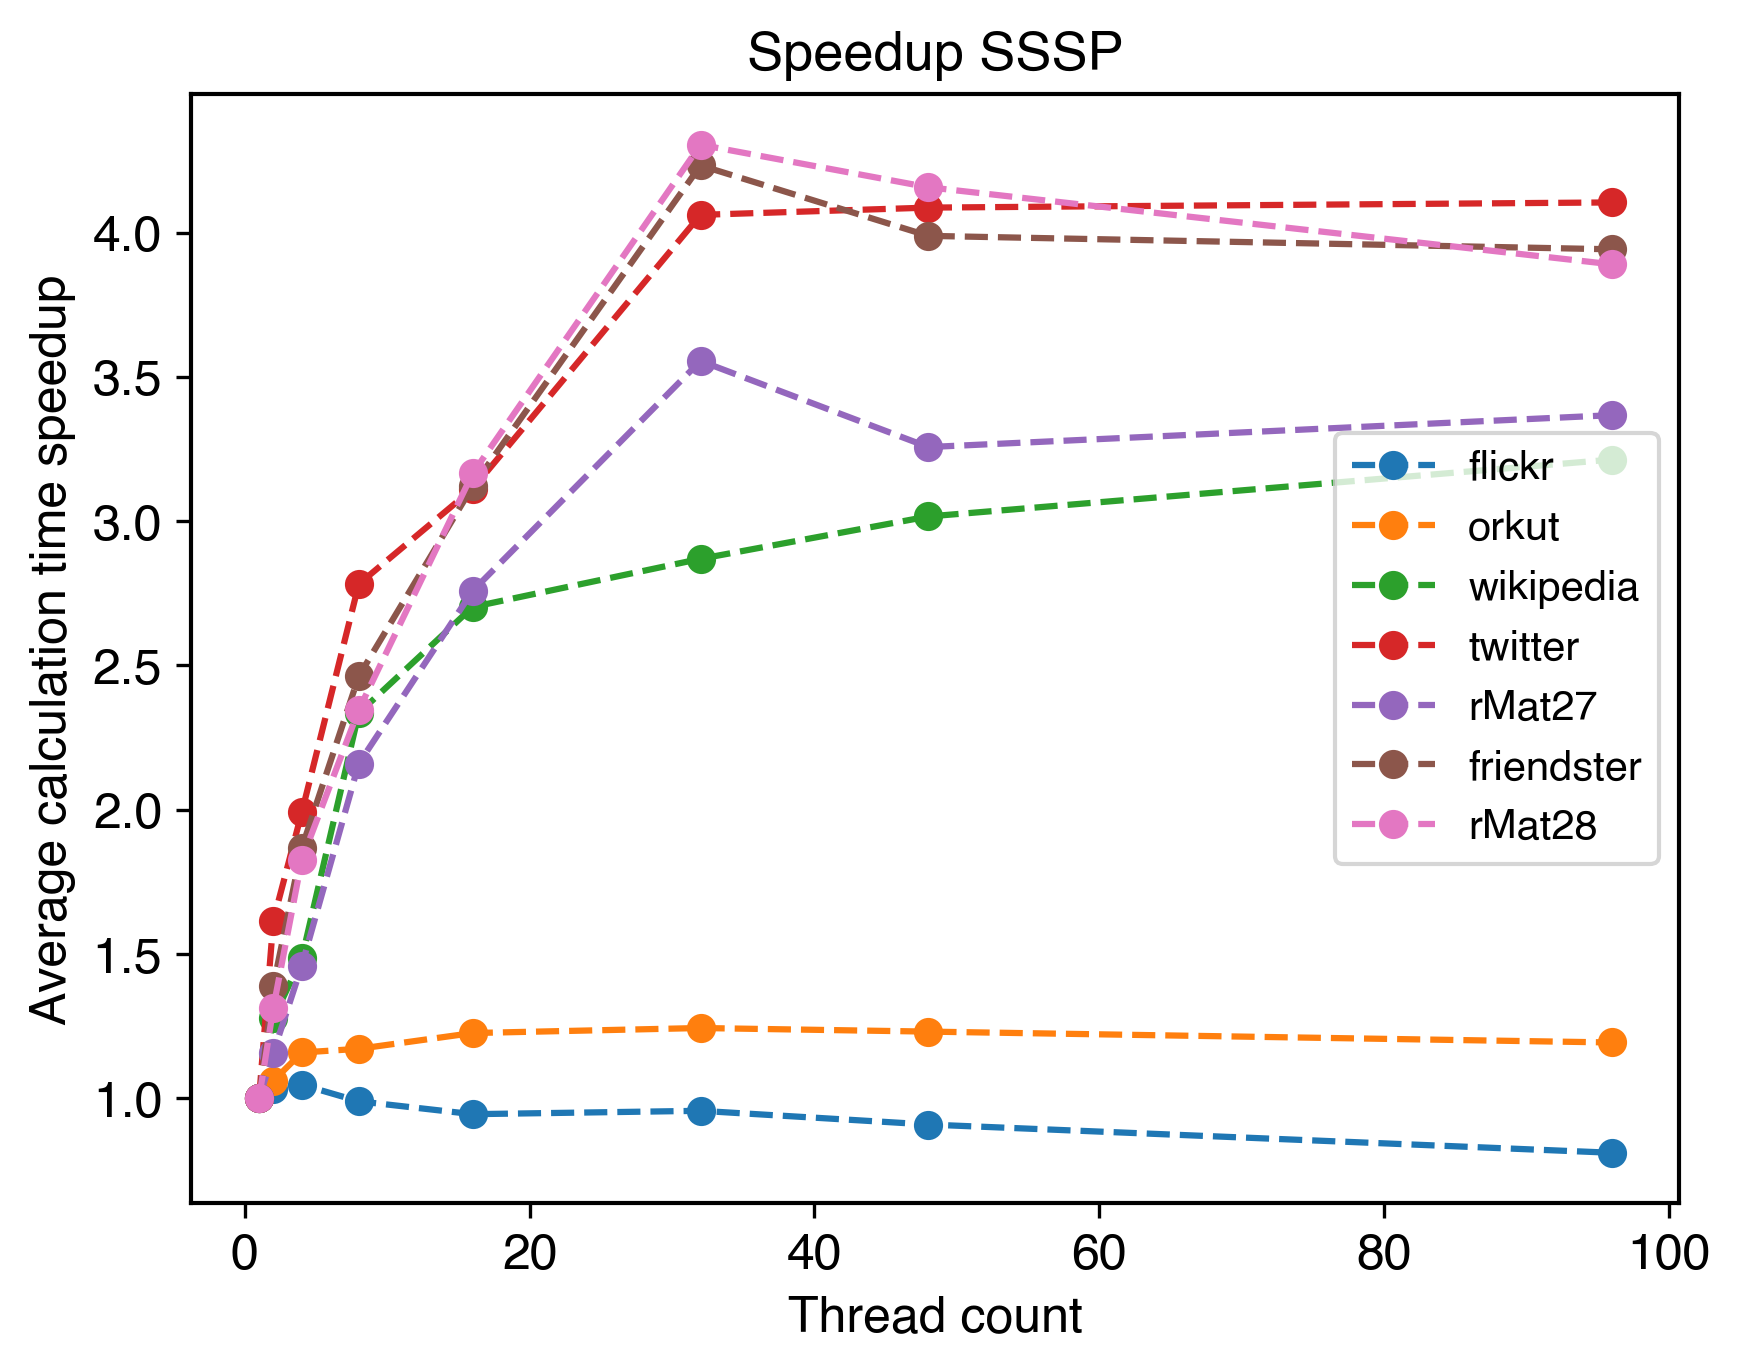
\includegraphics[width=\linewidth]{../../plots/singleNodeSSSPGaloisThreads.png}
		\caption{without hugepages}
		\label{fig:galoisSpeedupSSSP_noHP}
	\end{subfigure}
	\begin{subfigure}{0.4\textwidth}
		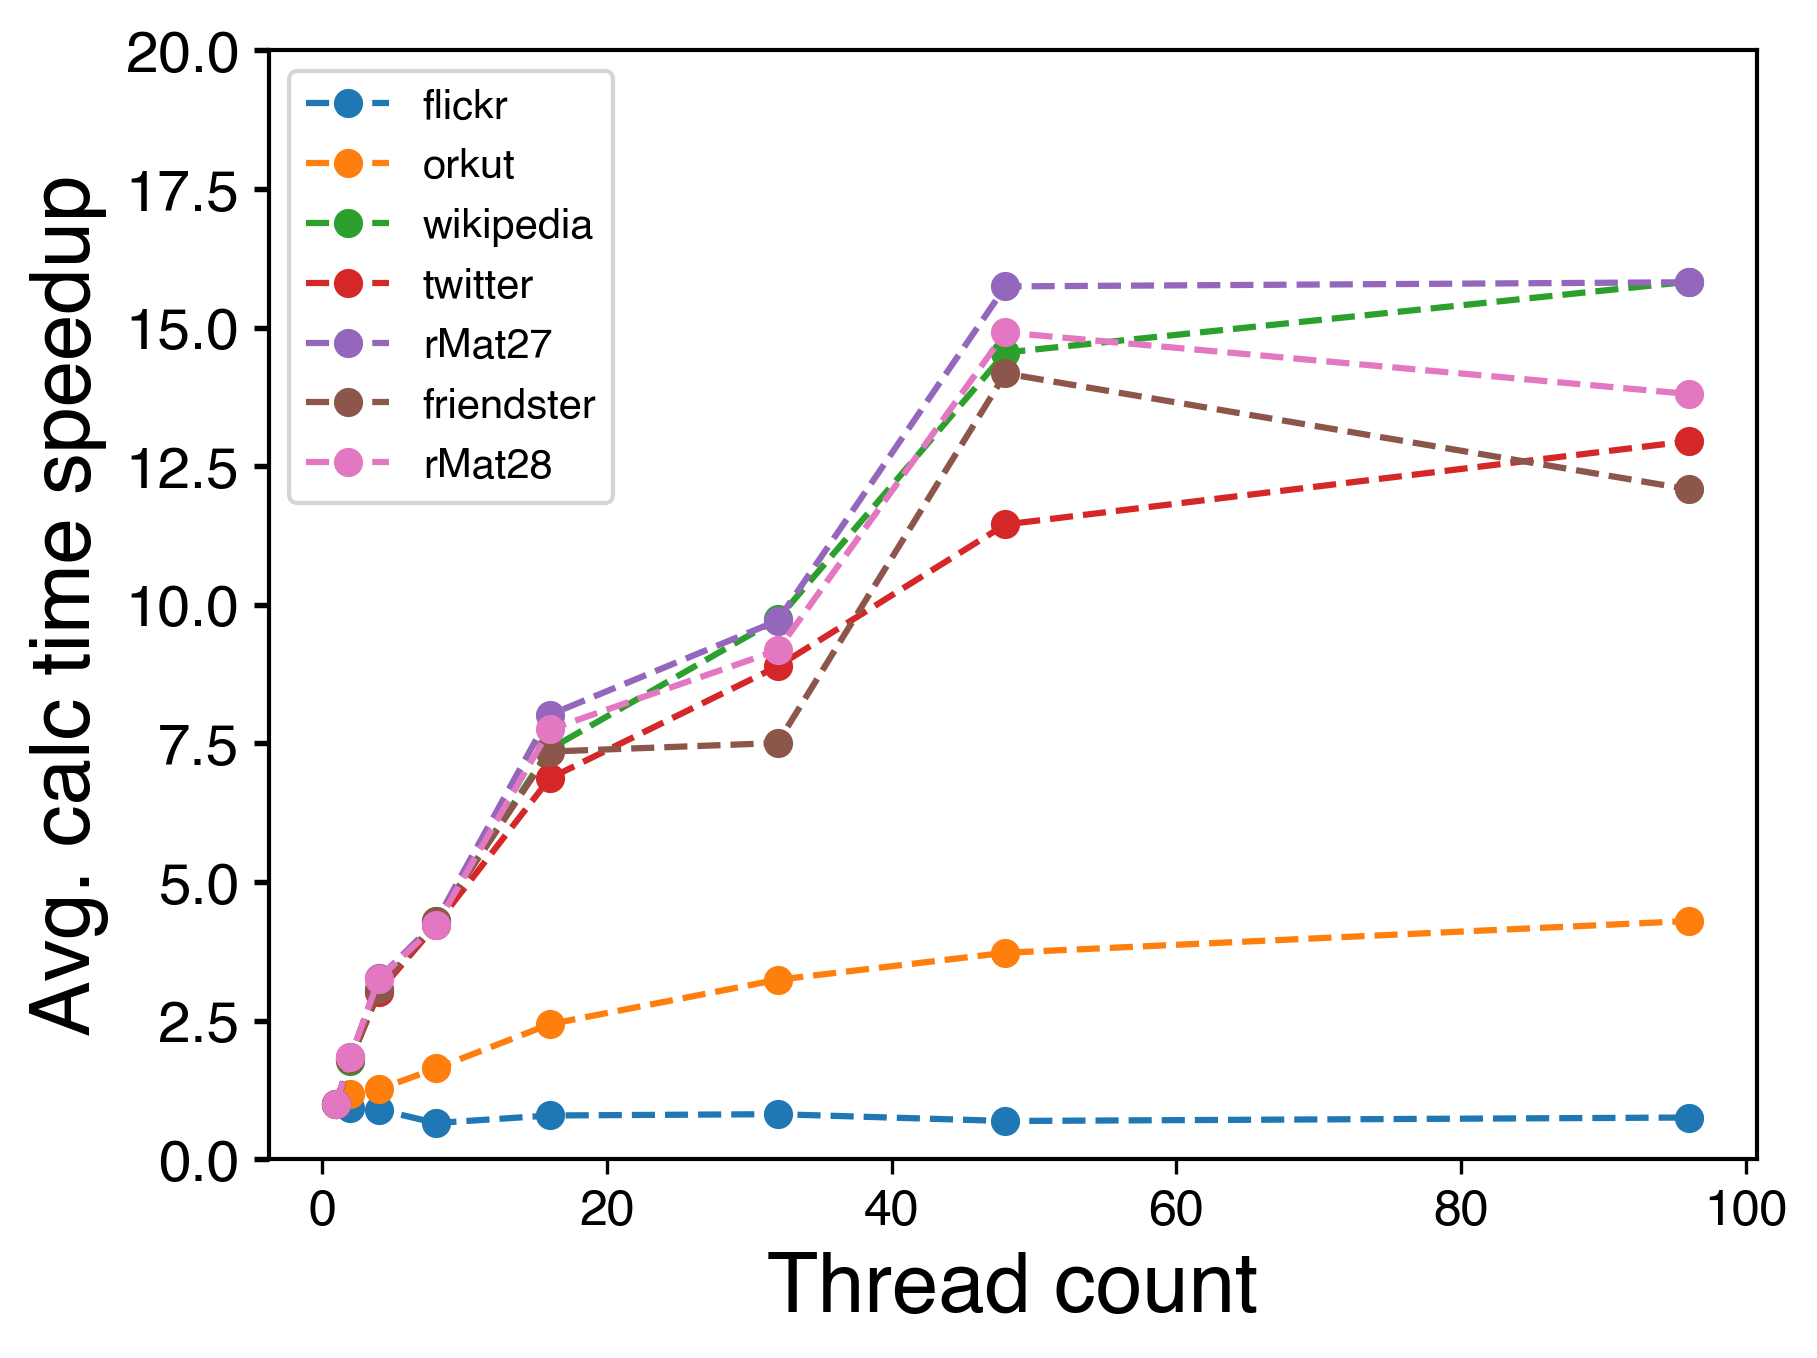
\includegraphics[width=\linewidth]{../../plots/singleNodeSSSPGaloisHPThreads.png}
		\caption{with hugepages}
		\label{fig:galoisSpeedupSSSP_HP}
	\end{subfigure}
	\hfil
	\caption{Calculation time speedups on SSSP}
	\label{fig:galoisSpeedupSSSP}
\end{figure*}
\begin{table}
\renewcommand{\arraystretch}{1.3}
\centering
\caption{Mean Speedups and Variances for SSSP With and Without HugePages}
\label{tbl:ssspMeansVariances}
\begin{tabular}{c
r@{\tabskip 1 \tabcolsep}r
r@{\tabskip 1 \tabcolsep}r}
\toprule
&\multicolumn{2}{c}{\!\!\!$\mu$}&\multicolumn{2}{c}{\!\!$\sigma^2$}\\
\cmidrule(r){2-3}\cmidrule(r){4-5}
{\bf\#Threads}&w/&w/o&w/&w/o\\\midrule
\bf1 & 1.0 & 1.0 & 0.0 & 0.0 \\
\bf2 & 1.6 & 1.6 & 0.2 & 0.1 \\
\bf4 & 2.5 & 2.5 & 1.1 & 0.9 \\
\bf8 & 4.5 & 3.4 & 5.3 & 2.1 \\
\bf16 & 6.7 & 5.8 & 13.0 & 7.3 \\
\bf32 & 9.6 & 7.0 & 38.3 & 10.8 \\
\bf48 & 10.3 & 10.7 & 41.4 & 31.4 \\
\bf96 & 10.2 & 10.8 & 38.1 & 29.9 \\
\bottomrule
\end{tabular}
\end{table}

Starting with SSSP, an algorithm that greatly benefits from many available threads. The results can be seen in \autoref{fig:galoisSpeedupSSSP}.
We first look at the speedups without hugepages, seen in \autoref{fig:galoisSpeedupSSSP_noHP}.
For all larger graphs, speedup is in most cases very close to optimal up to about 8 threads.
Twitter has the best speedup overall. It is 2.6$\times$ with 2 threads compared to one, 4$\times$ with 4, 7.7$\times$ with 8 and 9.7$\times$ using 16 threads.
Behaviour on friendster is similarly good. Here speedup is 1.9$\times$ at 2 threads compared to one, 3.5$\times$ at 4, 6.1$\times$ at 8 threads and 9.7$\times$ at 16 threads.
Anything above 16 threads however no longer helps decrease the computation time significantly on any graph. Speedup above 16 threads is always less than double the speedup of 16 threads. The maximum measured speedups are between 10$\times$ (96 threads, wikipedia) and 19$\times$ (40 threads, rMat28).
In some cases, increasing the thread count can even decrease the speedup again. For example calculation on rMat28 is actually slower with 48 or 96 threads compared to 40 threads. For 40 threads, the speedup is nearly 19$\times$, on 48 threads 17$\times$ and with 96 threads only 15$\times$ compared to one thread.
Small graphs, i.e. flickr and orkut neither benefit from more threads nor is the performance significantly held up by synchronization overhead.
Performance on flickr can not be sped up at all, with speedup on flickr being very close to 1 for 1 to 8 threads and between 0.7$\times$ to 0.9$\times$ from 16 to 96 threads.
Orkut reaches maximum speedup of 1.6$\times$ at 16 threads. But on orkut, the speedup is always greater or equal to 1.

Upon activating the hugepages, we acquired the results seen in \autoref{fig:galoisSpeedupSSSP_HP}. Here, the overall results are similar to the findings without hugepages. \autoref{tbl:ssspMeansVariances} shows the mean speedups and variances over the different graphs with and without hugepages. We see that the mean speedup is either very similar or slightly reduced by the hugepages. But in all cases with hugepages, the variance is significantly smaller. This proves a slightly smaller but more reliable speedup with hugepages.
Examples for this are on the one hand, orkut that could not reach a speedup above 1.6$\times$. Now, with hugepages it is 4.3$\times$ faster with 96 threads compared to one thread. On the other hand, twitter reached a speedup of 17$\times$ without hugepages and only 13$\times$ with.
While the hugepages did not neccessarily help improve the speedup value, they helped bring the different graphs together. 
Thus, the overall speedup benefit might not be as good as without hugepages. 
But the speedup is much more reliable regardless of the graph topology. 
In this regard, hugepages can be beneficial when many different graphs are in use, because it is more likely a speedup can be achieved. 
If only a few graphs are used, activating hugepages can decrease mutlithreaded performance, if the graphs behave for example like twitter above.

\paragraph{Breadth-First Search}
\begin{figure*}
	\hfil
	\begin{subfigure}{0.4\textwidth}
		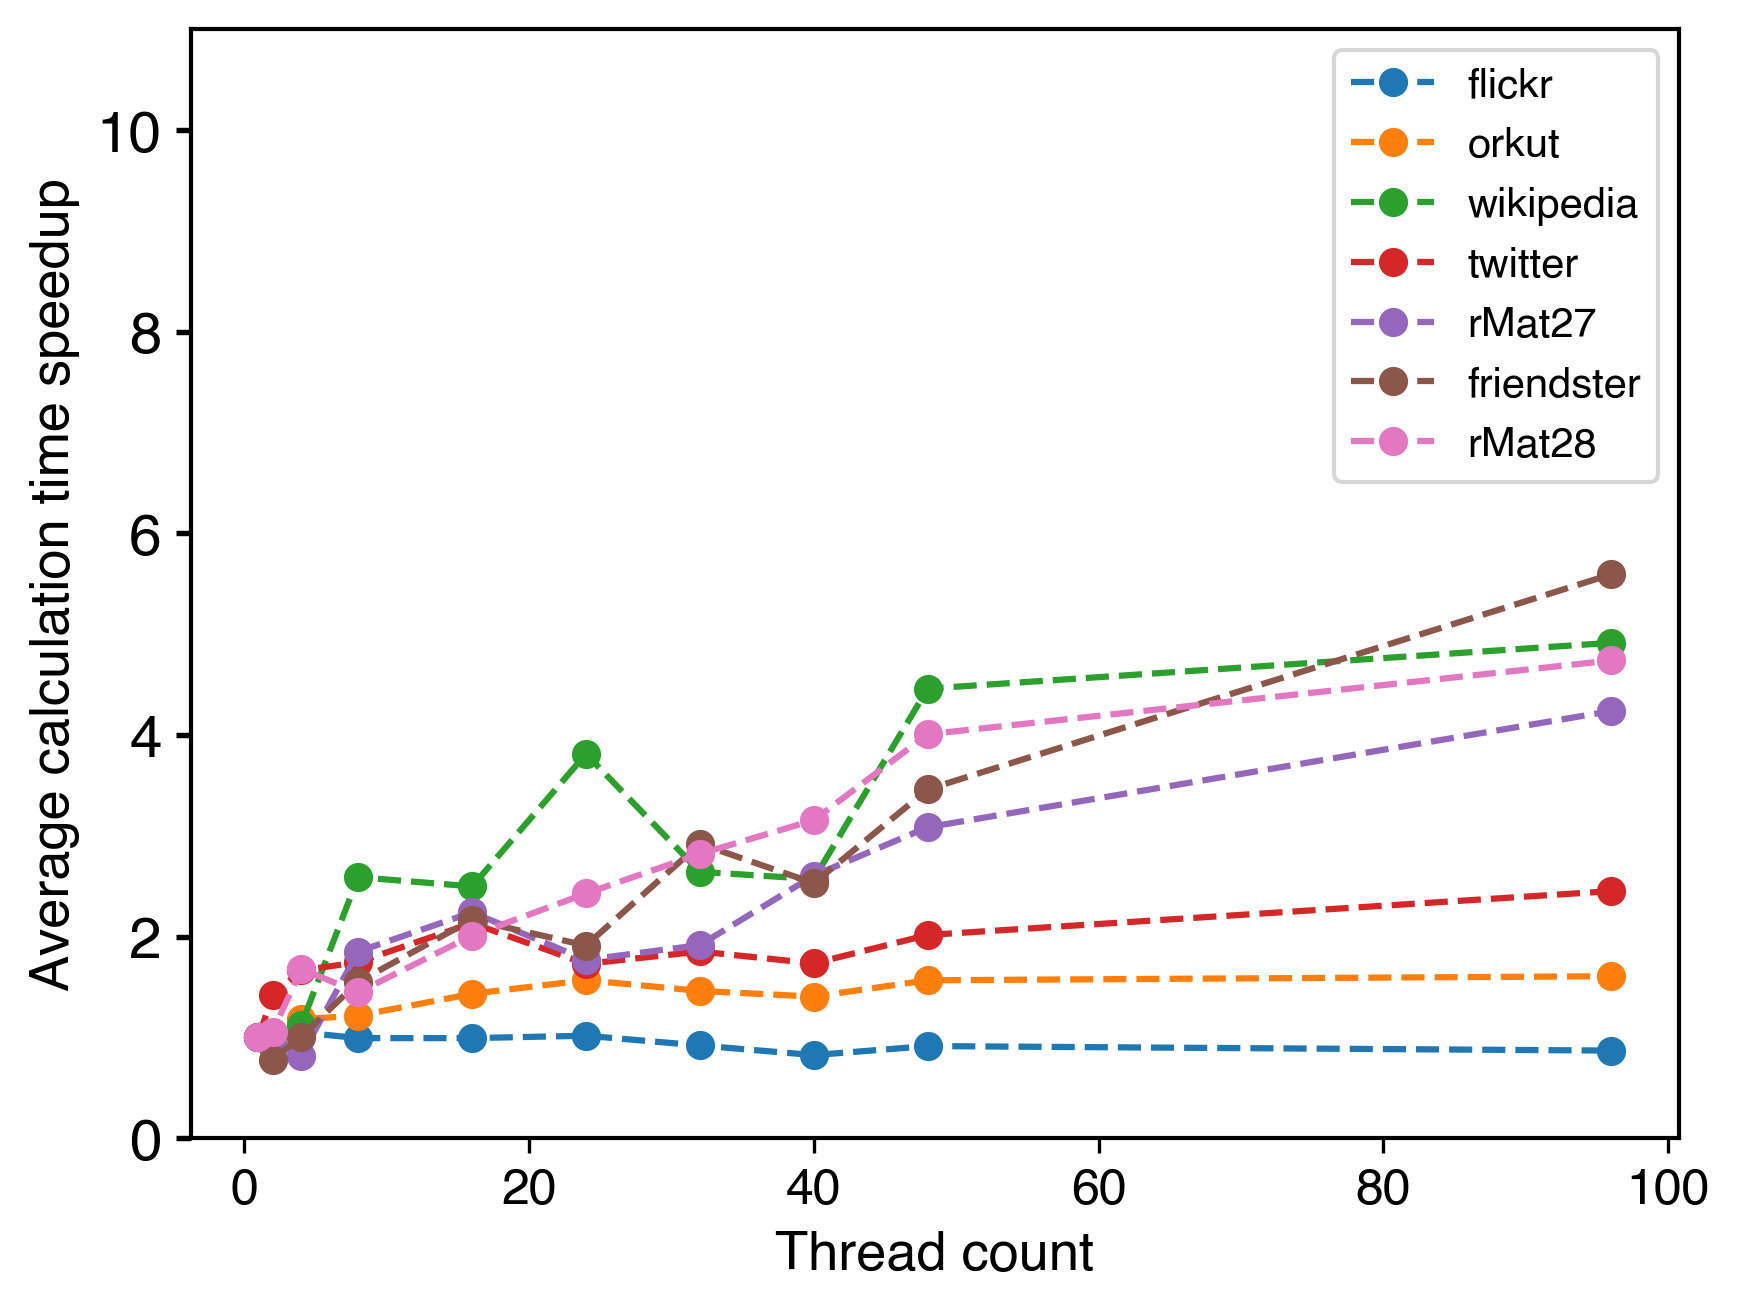
\includegraphics[width=\linewidth]{../../plots/singleNodeBFSGaloisThreads.png}
		\caption{without hugepages}
		\label{fig:galoisSpeedupBFS_noHP}
	\end{subfigure}
	\begin{subfigure}{0.4\textwidth}
		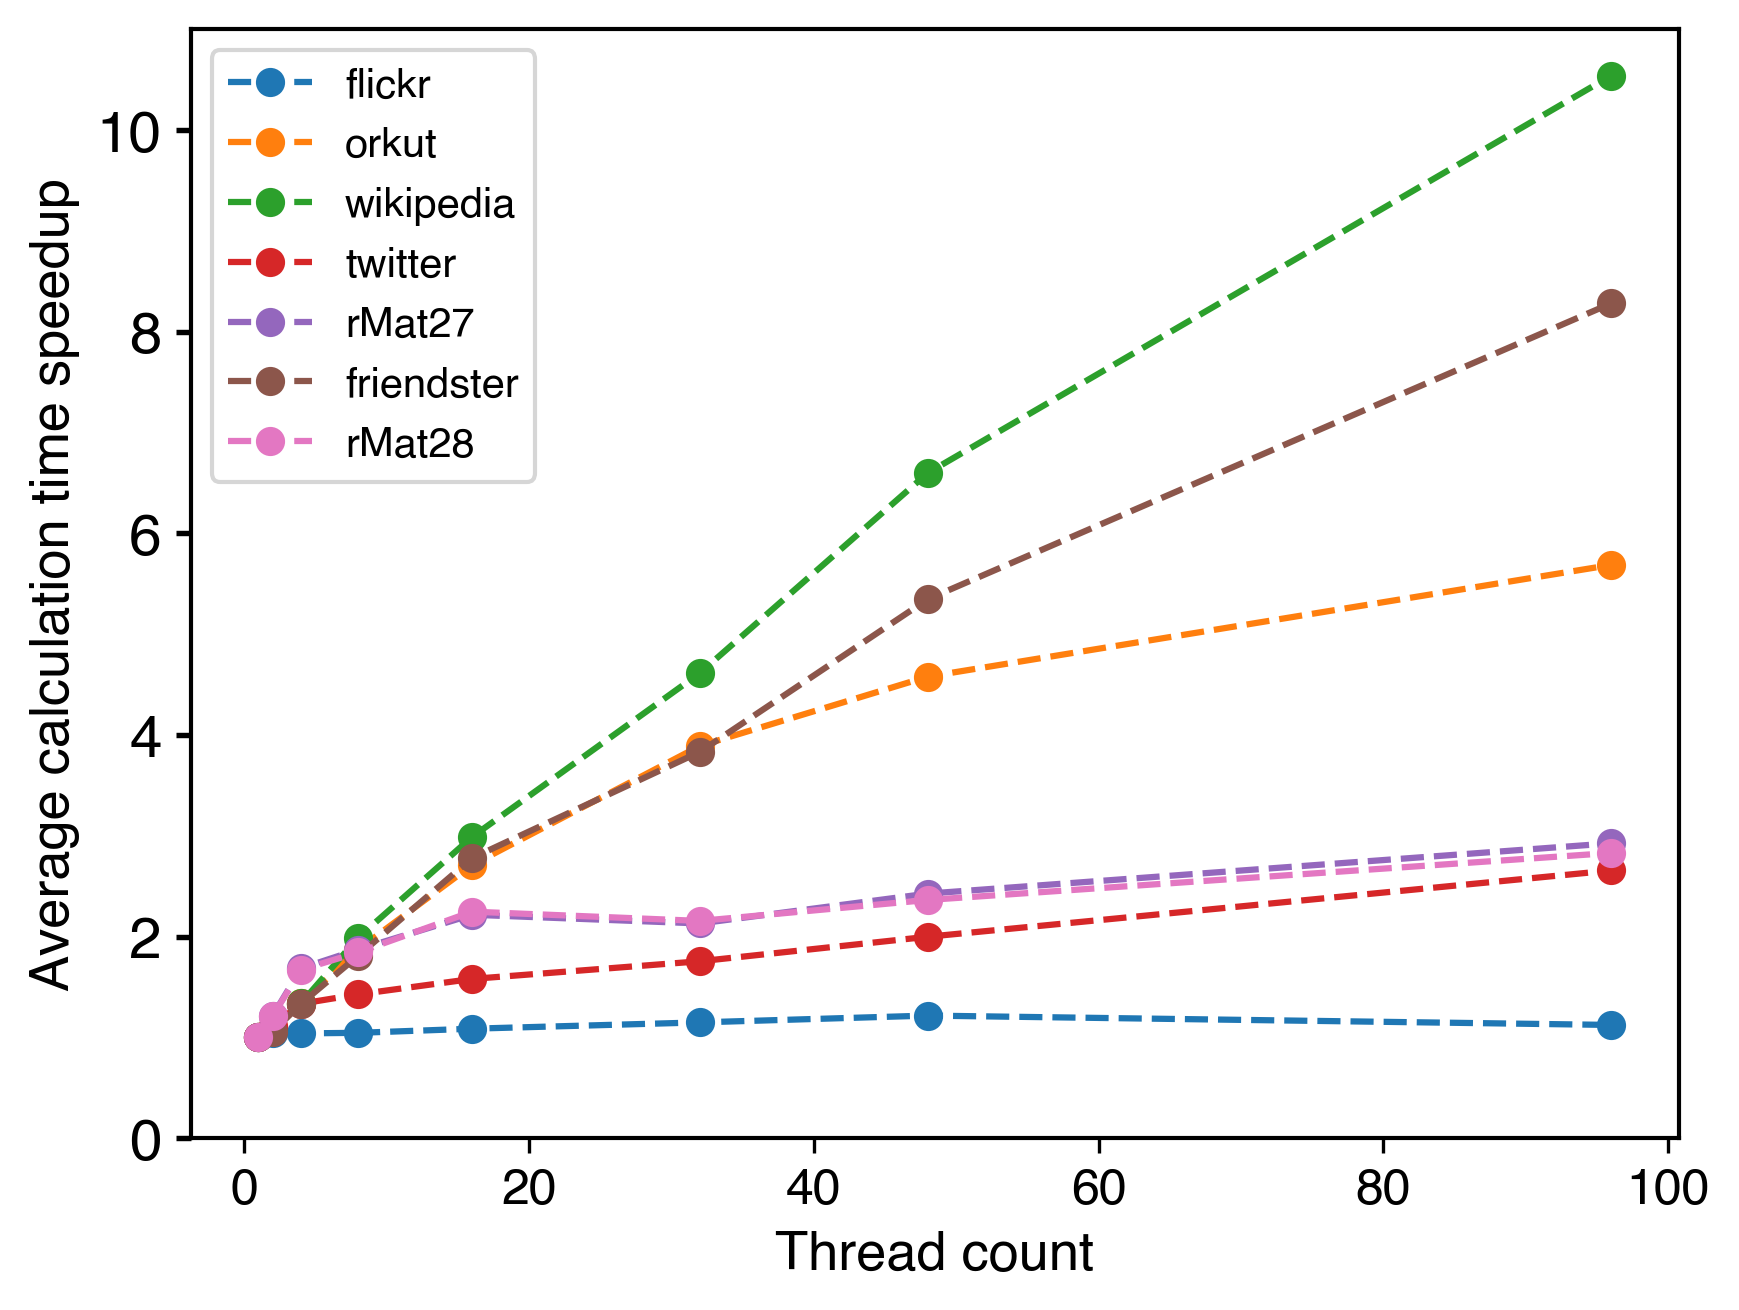
\includegraphics[width=\linewidth]{../../plots/singleNodeBFSGaloisHPThreads.png}
		\caption{with hugepages}
		\label{fig:galoisSpeedupBFS_HP}
	\end{subfigure}
	\hfil
	\caption{Calculation time speedups on BFS}
	\label{fig:galoisSpeedupBFS}
\end{figure*}

For our speedup results on BFS, \autoref{fig:galoisSpeedupBFS} shows the calculation time speedup of Galois' BFS with and without hugepages.
If we look at the results without hugepages first, we see most significantly, that the speedup never exceeds 6$\times$ even when using 96 threads (cf. \autoref{fig:galoisSpeedupBFS_noHP}).
For both flickr and orkut, we have the same behaviour as on SSSP without hugepages. Speedup is close to 1 in all cases, with orkut reaching a maximum speedup of 1.6$\times$ at 24 threads.
That said, the larger graphs are not benefitting from more threads as much as they did with SSSP. Twitter for example, reaches a speedup of 2$\times$ only with 48 or more threads. Meanwhile on SSSP, twitter reached a speedup of around 17$\times$ on those thread counts.
For the other graphs, the speedup is between 4.2$\times$ (rMat27) and 5.5$\times$ (friendster) at 96 threads. So while speedups are possible, not even remotely to the same degree as on SSSP. This, in turn is not intuitive, one would assume these two algorithms to perform similarly. Both algorithms are iterative traversal algorithms with comparable computation and synchronization complexity. But the worse speedup behaviour extends even to the case with hugepages (cf. \autoref{fig:galoisSpeedupBFS_HP}). While the results are generally better, still not to the same degree as on SSSP. With hugepages, BFS reaches a maximum speedup of 10.5$\times$ on wikipedia. The two graphs with largest speedup, namely wikipedia and friendster roughly follow a line with slope $1/8$. So with every 8 threads, the speedup is increased by about 1. Orkut follows the same line up to about 32 threads, slowly flattening off above that.
On the other graphs, a speedup of 3$\times$ is hardly reached, even at 96 threads.

\todo{Discussion ausarbeiten.. Was ist denn hier die Essenz, das ist ja beides irgendwie super schlecht.}

\paragraph{PageRank Pull}
\begin{figure*}
	\hfil
	\begin{subfigure}{0.4\textwidth}
		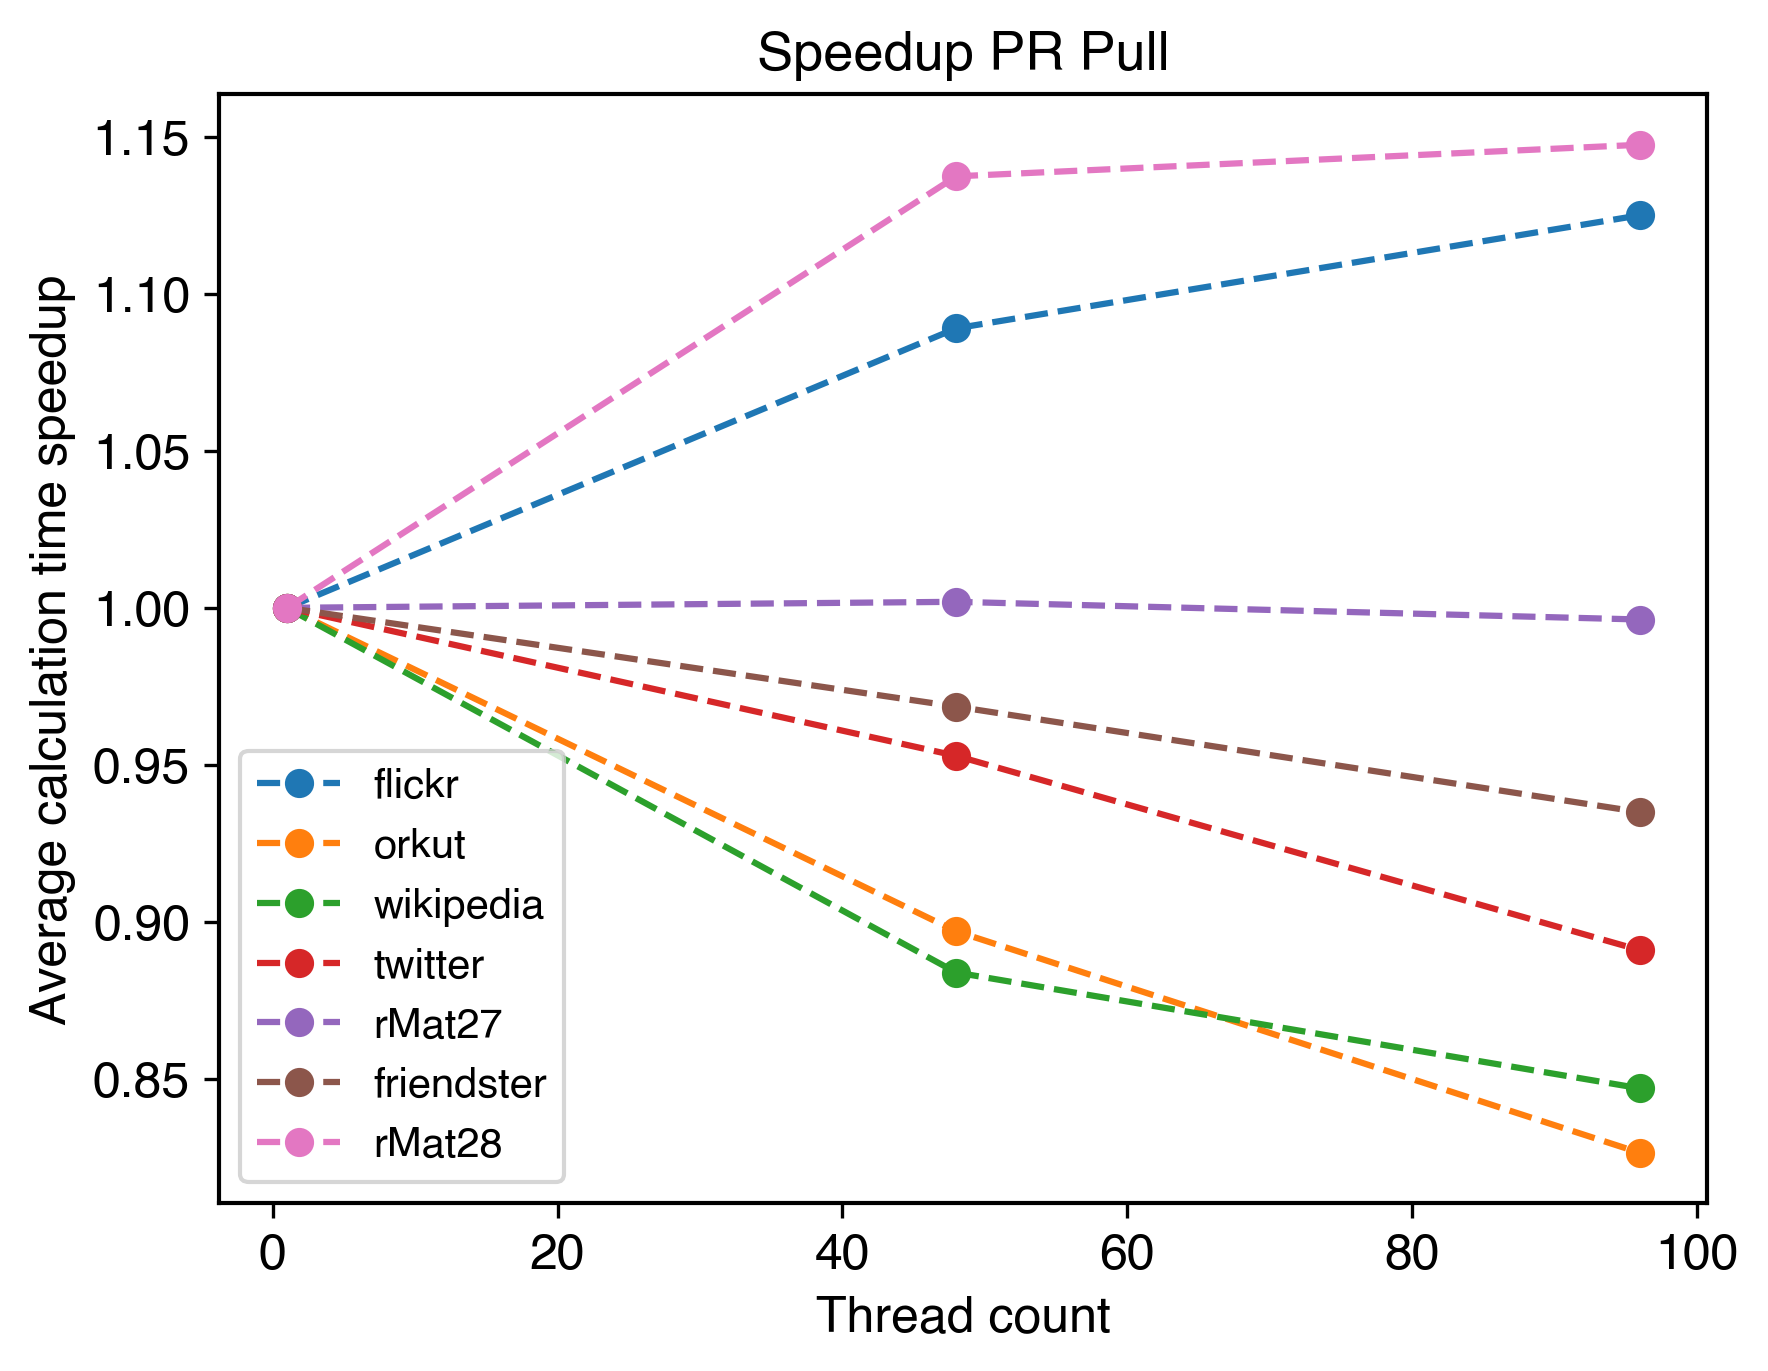
\includegraphics[width=\linewidth]{../../plots/singleNodePRPullGaloisThreads.png}
		\caption{without hugepages}
		\label{fig:galoisSpeedupPRPull_noHP}
	\end{subfigure}
	\begin{subfigure}{0.4\textwidth}
		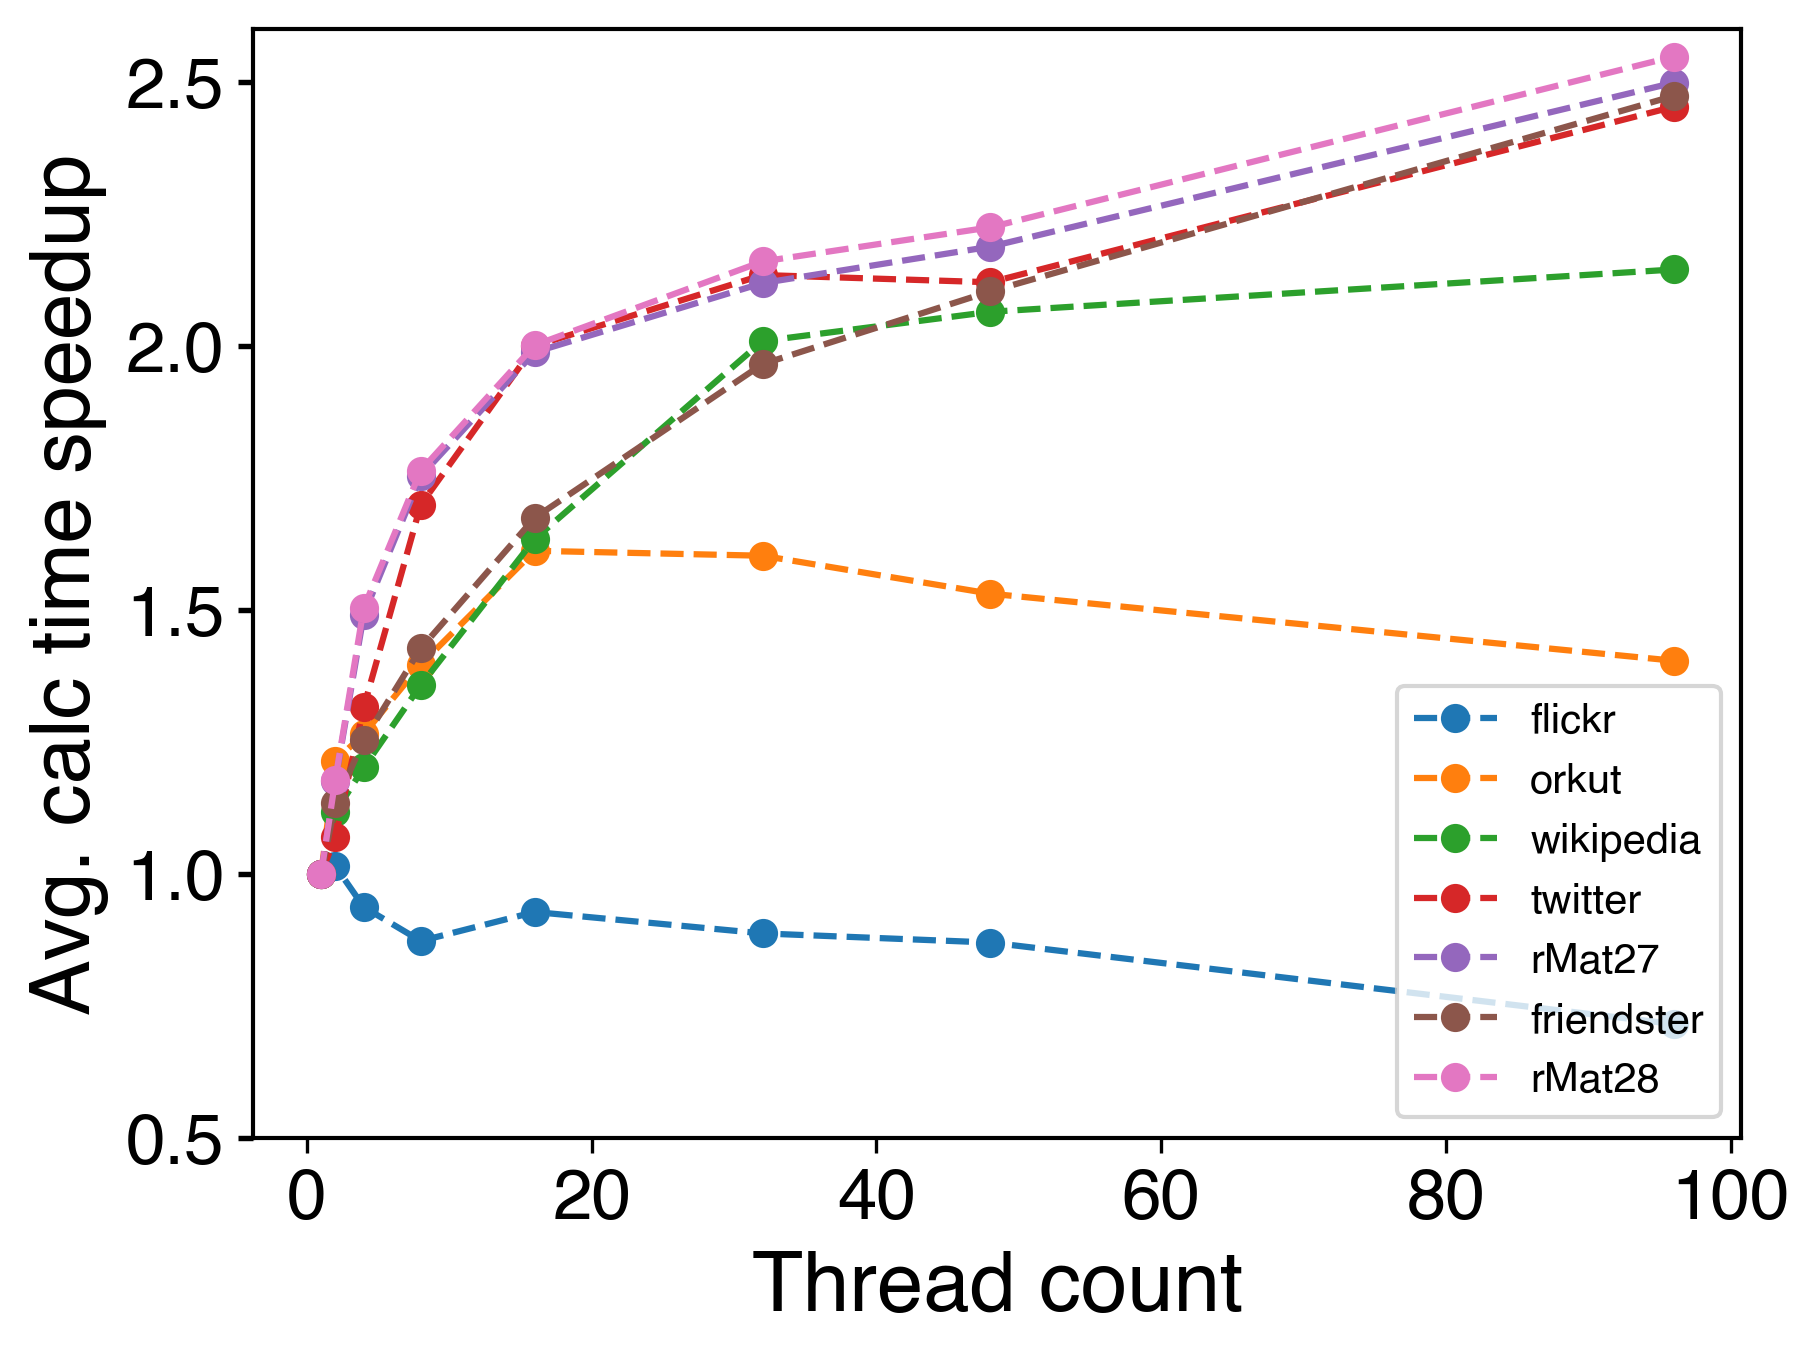
\includegraphics[width=\linewidth]{../../plots/singleNodePRPullGaloisHPThreads.png}
		\caption{with hugepages}
		\label{fig:galoisSpeedupPRPull_HP}
	\end{subfigure}
	\hfil
	\caption{Calculation time speedups on PR Pull}
	\label{fig:galoisSpeedupPRPull}
\end{figure*}

We want to first take a look at the results for PageRank in Pull mode, seen in \autoref{fig:galoisSpeedupPRPull}. Without hugepages, computation time is hardly reduced on any graph other than flickr, where the reached maximum is 1.6$\times$ (cf. \autoref{fig:galoisSpeedupPRPull_noHP}). This maximum is reached at two threads, with speedup steadily declining above that.
The rMat28 is the only other graph of one could say computation was sped up at large thread counts. Here we reached a maximum speedup of 1.3$\times$ at 96 threads.
All 5 other graphs only reach a speedup greater or equal to 1 in just one or two cases, and if so only by a small margin.
Computation on Orkut and Twitter reaches a speedup maximum of 1.1$\times$ and 1.05$\times$ at 4 threads, while being less or equal to 1 in all other cases.
Speedup on the wikipedia graph is never grater than one.
Friendster and rMat27 can be sped up to 1.07$\times$ or 1.1$\times$ respectively on 8 threads.

Most of this changes drastically with the activation of hugepages, our data can be seen in \autoref{fig:galoisSpeedupPRPull_HP}. 
Here actually all graphs except flickr reach a speedup greater than 1.5$\times$. Remember, that 1.6$\times$ was the maximum possible speedup without hugepages.
Furthermore, orkut is the only graph that never reaches a speedup of 2$\times$.
Twitter, rMat27, friendster and rMat28 all reach a speedup of around 2.5$\times$ at 96 threads.

We conclude hugepages to be very much recommended for any pull based algorithm similar to PageRank (or PR itself).
Only with hugepages enabled do we observe a considerable increase in performance and thus a benefit of utilizing many threads.
Without hugepages tough, having many threads available is in most cases slowing down performance.

\todo{Discussion ausarbeiten}

\paragraph{PageRank Push}
\begin{figure*}
	\hfil
	\begin{subfigure}{0.4\textwidth}
		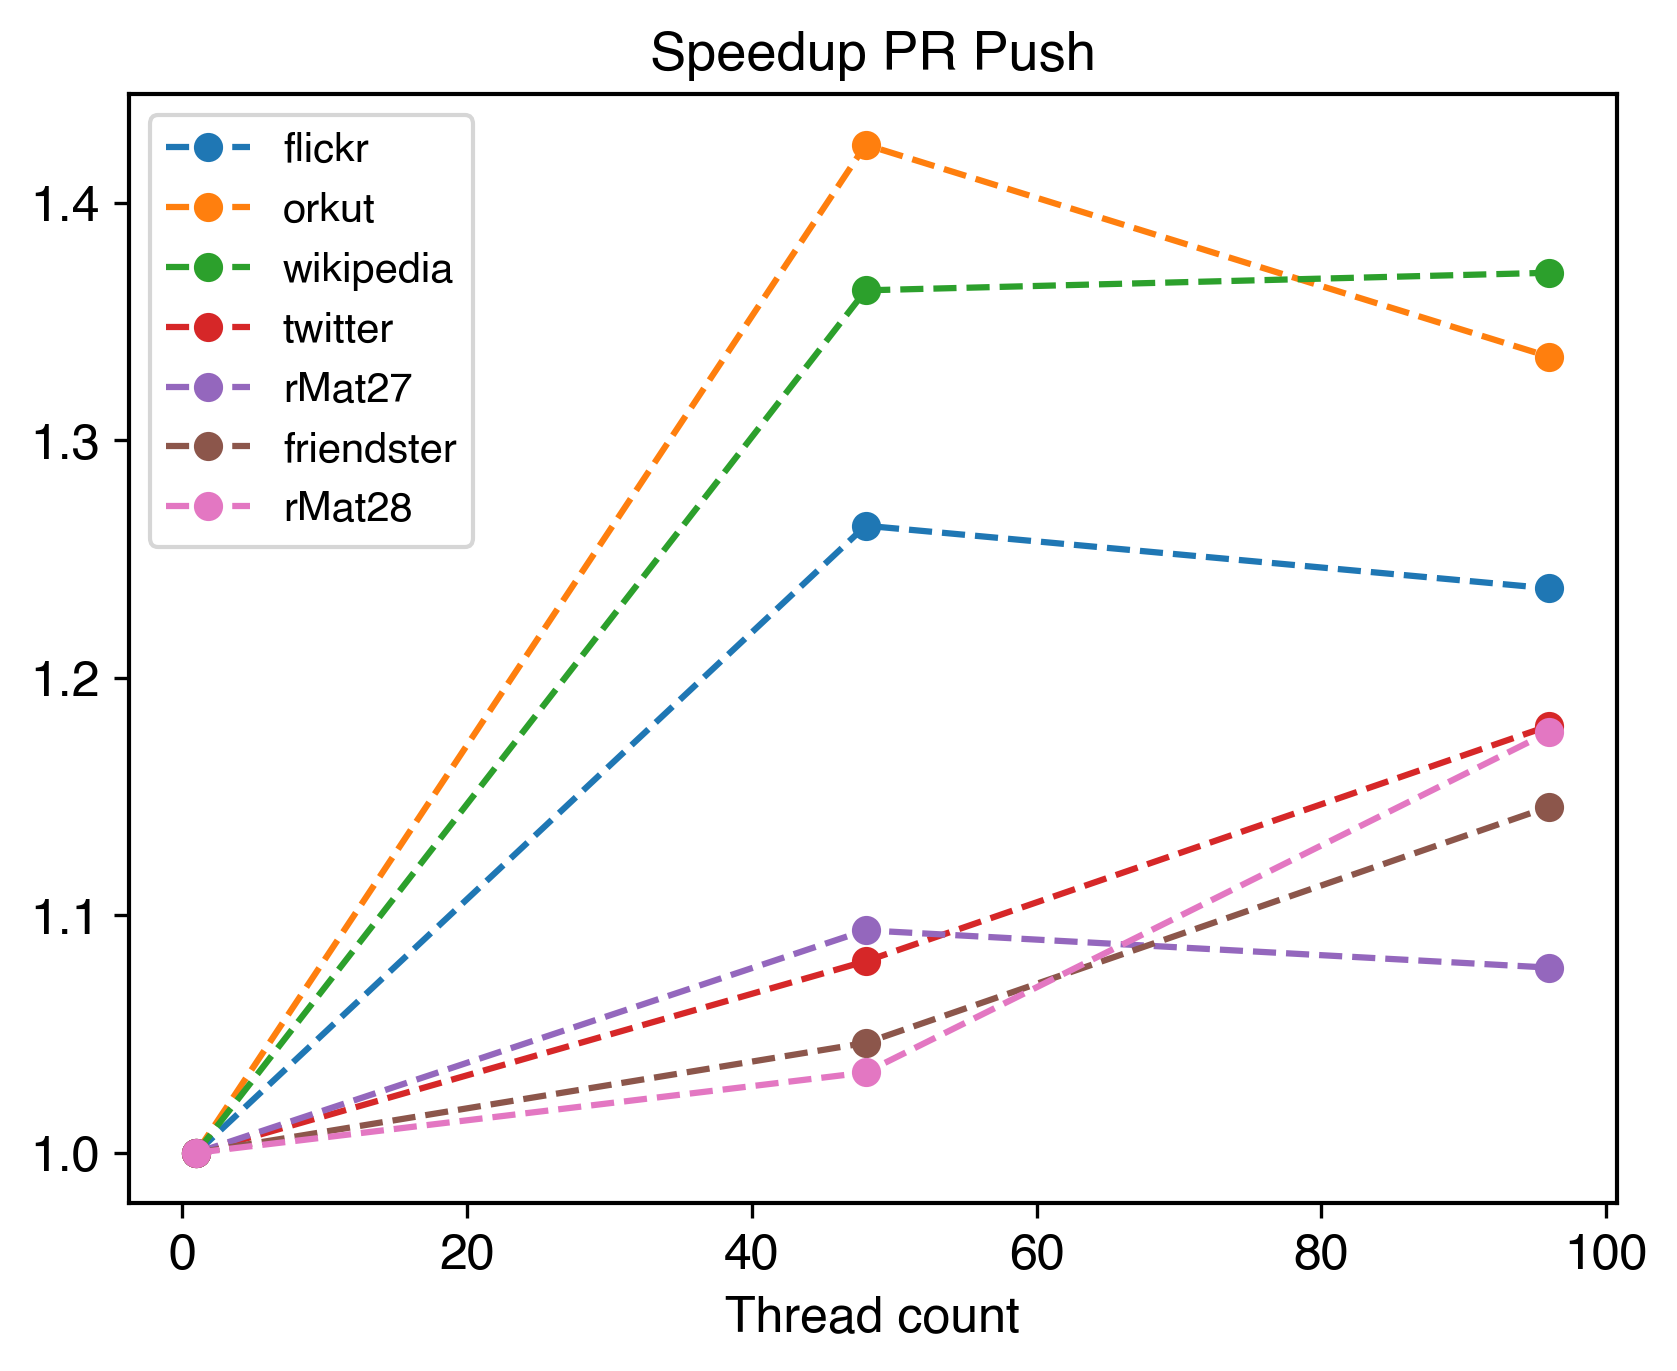
\includegraphics[width=\linewidth]{../../plots/singleNodePRPushGaloisThreads.png}
		\caption{without hugepages}
		\label{fig:galoisSpeedupPRPush_noHP}
	\end{subfigure}
	\begin{subfigure}{0.4\textwidth}
		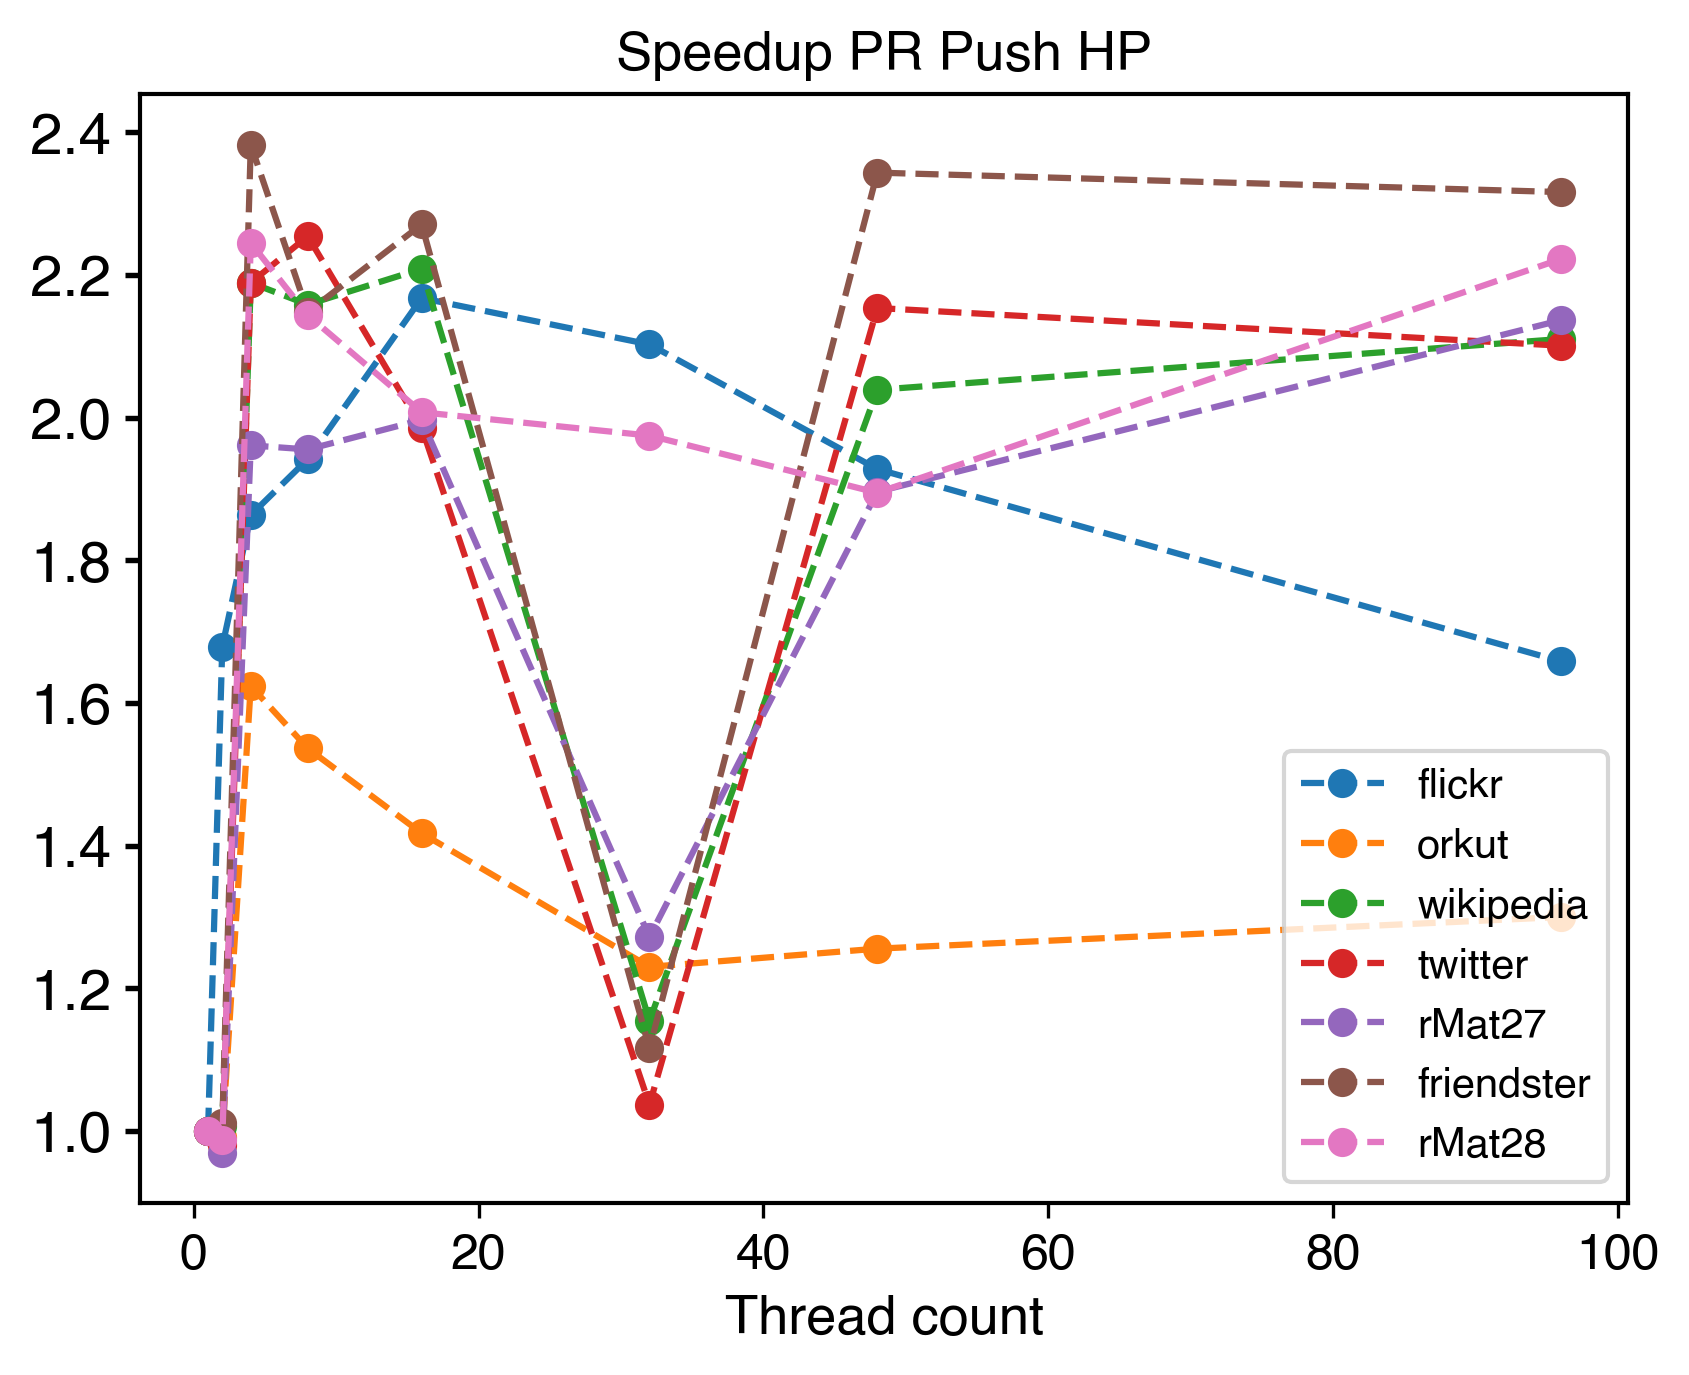
\includegraphics[width=\linewidth]{../../plots/singleNodePRPushGaloisHPThreads.png}
		\caption{with hugepages}
		\label{fig:galoisSpeedupPRPush_HP}
	\end{subfigure}
	\hfil
	\caption{Calculation time speedups on PR Push}
	\label{fig:galoisSpeedupPRPush}
\end{figure*}

The speedup results on the Push variant show odd behaviour in the Galois implementation, both with and without hugepages.
Especially without hugepages though, there is a significant performance loss on 4, 24 and 40 threads that is far from the expected behaviour. This is most visible in \autoref{fig:galoisSpeedupPRPush_noHP}, we validated the shown results with multiple samples each.
The speedup for 24 threads is, by interpolating between 16 and 32 threads, expected to be anywhere between 1.3$\times$ and 1.9$\times$.
Actually however, the system does not reach a speedup of more than 1.04$\times$ on any graph, with only rMat27 actually reaching a value greater than 1.
On all other graphs, using 24 threads is anywhere from 3\% (flickr) to 9\%\ (wikipedia) slower than using just one thread.
We intially assumed that this is due to the missing hugepages, Galois is recommended to be run with. This seems to be only partly true, since the results with hugepages are generally better, but still show some of this behaviour (cf. \autoref{fig:galoisSpeedupPRPush_HP}).
There is only one significant anomaly at 32 threads, while the points where we observed the performance drop without hugepages look more \emph{reasonable}\todo{das ist nicht das wort das ich suche..}.
At 32 threads, speedup for 5 of 7 graphs drops to a value between 1.4$\times$ and 1.5$\times$. Yet those five graphs reach a speedup larger than 1.8$\times$ both at 16 and 48 threads (i.e. immediately before and after 32).

Nevertheless, if we disregard these anomalies, we see a significant performance increase with hugepages compared to without them. Actually, all graphs show an improvement in their maximum reached spedups. The largest improvements are from 1.5$\times$ to 2.1$\times$ for rMat27, 1.5$\times$ to 2.4$\times$ for friendster and 1.4$\times$ to 2.2$\times$ for rMat28, just by switching hugepages on.
Interestingly, with hugepages all graphs reach a speedup at 4 threads that is very similar, if not equal to the speedup at 96 threads. The largest discrepancy between the two thread counts is rMat27, with a performance uplift from 1.96$\times$ to 2.14$\times$ at 4 and 96 threads.

Using hugepages shows very effective, while it does not completely remove the anomalies we observed, it definitely increases performance by a considerable margin.

But, at least on our testing data, more than 4 threads did not change the performance significantly.
\todo{Discussion ausarbeiten}
